The wetting theory describes the interaction of fluids with solid surfaces. Many processes in nature, as well as in technology, are affected by this phenomenon. In this work, the focus is on the wetting properties in capillaries, which are often used as a simplification for understanding porous media or in other processes, such as the fact that trees would not be as tall as they are today without this effect. \todo{mention that we are considering spontaneous cap rise (no pressure or something like that)}

First, an overview of some types of wetting is presented \todo{ref}, and the concepts of contact angle and contact line are introduced. Subsequently, the surface tension \todo{ref} and its role in wetting are discussed. Since this work considers the dynamic rise of a water column in a capillary, the dynamic contact angle is also examined in Chapter \todo{ref chapter}, followed by a description of the capillary effect \todo{ref} and its significance for the rise of a fluid in a capillary. \todo{rework}

\section{Surface Tension}
\label{sec: Wetting_SurfaceTension}
Surface tension plays a significant role in the wetting of surfaces or in capillary rise. Therefore, it is essential to first clarify what surface tension is. In general, surface tension is a proportionality constant that depends on temperature, pressure, and the phases involved but is independent of the surface \cite{buttPhysicsChemistryInterfaces}. The interface separates the phases and can be interpreted differently. \todo{possibly ref to corresponding chapters here.}
On a molecular level, molecules attract each other (cohesion). The interaction between two phases is called adhesion. In the case of the interaction between a liquid and a solid, adhesion can usually be neglected. In Figure \ref{fig: WettingTheory_SurfaceTensionMolecules}, a water droplet surrounded by air is illustrated on the left. The black outer line thus represents the interface between the droplet and the air. If one now magnifies the transition area down to the molecular level (red area), one obtains the schematic representation on the right side. The blue circles are simplified representations of the water molecules, and the gray ones represent the surrounding air. Here, it is evident how, at the interface, the water molecules are no longer surrounded only by other water molecules, which is energetically unfavorable. However, since the system strives to transition into an energetically favorable state, it attempts to minimize the number of molecules lying at the interface \cite{buttPhysicsChemistryInterfaces}.

\begin{figure}[h]
    \centering
    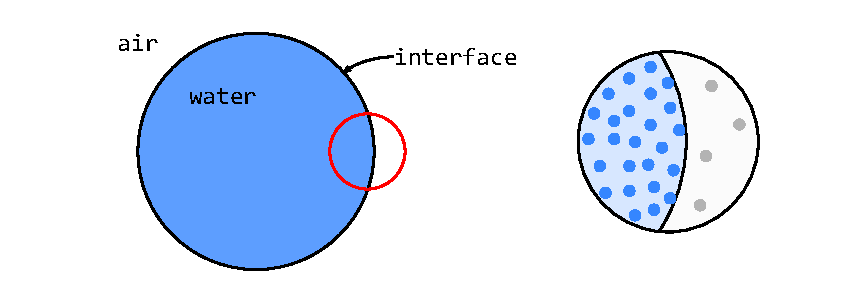
\includegraphics[width=.9\textwidth]{Pictures/moleculesAhesionCohesion_Wetting.pdf}
    \caption{Schematic of interacting molecules in a liquid droplet and its interaction with a vapor}
    \label{fig: WettingTheory_SurfaceTensionMolecules}
\end{figure}
To increase the surface area, molecules must be transported to the surface, and energy must be supplied to the system. Therefore, surface tension is also interpreted as the necessary energy required to carry a molecule to the surface.
\begin{equation}
 dE = \sigma \cdot dA
\end{equation}
with \(dE\) as the supplied energy and \(dA\) as the change in surface area.


\section{Wetting Phenomenon}
Despite the fact that the wetting of droplets is not considered in this work, it is appropriate to describe the fundamentals of wetting using this example. The concepts are the same, and many initial studies are based on this example.

In the case where the system is in equilibrium, Young \todo{ref} derived an equation relating surface tensions to the contact angle:
\begin{equation}
    \sigma_{LV} \cdot \cos\theta_e = \sigma_{SV}-\sigma_{SL}
    \label{eq: YoungsEQ}
\end{equation}
Where $\sigma_{LV}$ is the surface tension between the liquid and the gas, $\sigma_{SV}$ is from the solid to the gas, and $\sigma_{SL}$ is between the solid and the liquid (see Figure \ref{fig: YoungsLaw_ThreePhaseContactLine}).
\begin{figure}[h]
    \centering
    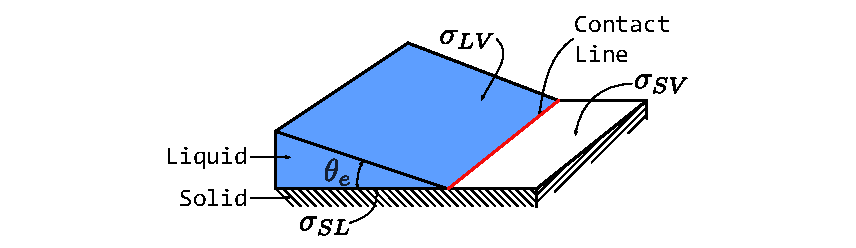
\includegraphics[width=.9\textwidth]{Pictures/YoungsLaw.pdf}
    \caption{Three Phase Contact Line}
    \label{fig: YoungsLaw_ThreePhaseContactLine}
\end{figure}
If $(\sigma_{SV}>\sigma_{SL})$ holds true, a contact angle less than $90°$ follows; otherwise, $90°\leq \theta_e<180°$. In the case where $\sigma_{SV}=\sigma_{SL}+\sigma_{LV}$, complete wetting of the surface occurs \cite{buttPhysicsChemistryInterfaces}.

When a droplet impacts a solid surface, different states can arise depending on the fluid-solid combination. At the point where the interface of the two fluids (droplet and surrounding fluid) meets the solid surface, the contact line is formed (see \ref{fig: YoungsLaw_ThreePhaseContactLine}; red line). Depending on the fluid-fluid-solid combination, a contact angle $\theta_e$ is established, where the suffix $e$ stands for equilibrium. In the case of complete wetting, the fluid spreads over the entire surface (see Figure \ref{fig: WettingTheory_WettingOfSurface} a)). This effect, however, is challenging to reproduce as it can be hindered by surface irregularities \todo{ref; i think it was butt}. As seen in Figure \ref{fig: WettingTheory_WettingOfSurface}(b-d)), states where a droplet forms on the surface are further subdivided. For a contact angle $\theta_e<90°$, it is termed hydrophilic (see \ref{fig: WettingTheory_WettingOfSurface}b)), for $\theta_e>90°$ it's hydrophobic (see \ref{fig: WettingTheory_WettingOfSurface}c)), and for a contact angle $\theta_e>120°$, it's superhydrophobic surfaces (see \ref{fig: WettingTheory_WettingOfSurface}d)). Developing superhydrophobic surfaces is also challenging.
\begin{figure}[h]
    \centering
    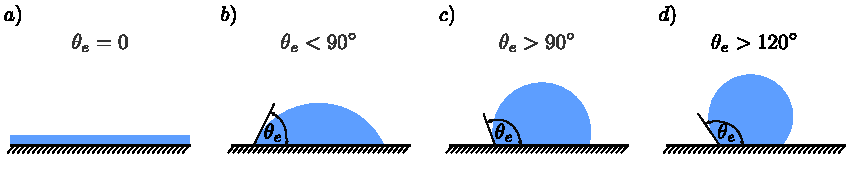
\includegraphics[width=.95\textwidth]{Pictures/DropletsAndWetting.pdf}
    \caption{Wetting of a surface}
    \label{fig: WettingTheory_WettingOfSurface}
\end{figure}
To curve the surface of the liquid, a pressure difference must exist. In the case of a sphere, Young and Laplace developed a relationship for the pressure difference in terms of the surface tension and radius as:
\begin{equation}
\label{eq: YoungLaplaceEQ}
    P_i - P_o = \Delta P =  \frac{2\sigma}{R}
\end{equation}
With $\Delta P$ being the pressure difference at the interface, $P_i$ as the pressure inside the droplet, $P_o$ the ambient pressure, and $R$ as the radius of the sphere. For a derivation, refer to \cite{buttPhysicsChemistryInterfaces}.
\subsection{Dynamic Wetting}
So far, only equilibrium states have been considered. Typically, however, the contact line is in motion. When the contact line is moving, the contact angle (dynamic contact angle $\theta_D$) differs from that in equilibrium \cite{blake2006PhysicsMovingWetting}. To describe the dynamics of the contact line, the dynamic contact angle, the relative speed of the contact line, and the equilibrium contact angle are required \cite{mohammadkarim2022ReviewPhysicsMoving, blake2006PhysicsMovingWetting, cox1986DynamicsSpreadingLiquids, huh1971HydrodynamicModelSteady, voinovHydrodynamicsWetting1977}.
Describing the contact line is challenging due to the influence of the microscopic level on the macroscopic level. Therefore, the phase field method requires both hydrodynamic approaches and molecular kinetic theory approaches \cite{blake2006PhysicsMovingWetting, carlsonCapillarityDynamicWetting2012}.
The hydrodynamic approach solves the physics of flow using the Navier-Stokes equations but encounters a singularity at the contact line when applying the adhesion condition. To address this issue, the adhesion condition near the wall has been relaxed, or the solution at the molecular level has been truncated \cite{blake2006PhysicsMovingWetting}.
\begin{figure}[h]
    \centering
    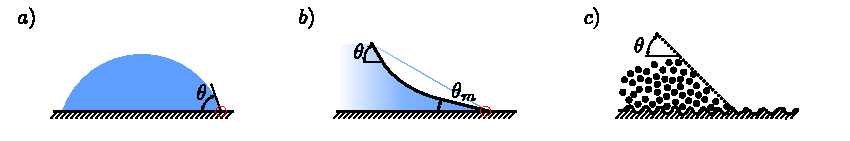
\includegraphics[width=.95\textwidth]{Pictures/ContactAngles_HDT_MKT.pdf}
    \caption{Hydrodynamic and Molecular Kinetic description of the Contact angle. Figure b) corresponds to the area circled in red in a), and c) to the image from b).}
    \label{fig: HDT_MKT_comp}
\end{figure}
The Molecular Kinetic Model describes the motion of the contact line with a statistical description of molecular motion at the contact line \cite{blake1969KineticsDisplacement}. Unlike the hydrodynamic model, molecular processes at the contact line influence larger scales. In this view, molecules at the contact line jump back and forth to adsorption sites on the solid substrate. When the system is in equilibrium, the jumping is balanced, and the contact line comes to a halt \cite{car, blake2006PhysicsMovingWetting}. However, a challenge with this approach is that this model is more qualitative and computationally intensive. \todo{probably a bad end of the chapter}.

The phase field theory uses approaches from both models, utilizing the description of the system's free energy. \todo{ref chapter PhaseField}

\todo[inline]{the following maybe in the bib rev? I'm writing about it there, but briefly. Maybe more detail there and skip it here? I dunno}
\section{Capillary Rise}
In previous chapters, droplets on solid surfaces were used to describe the dynamics of the contact line. These insights can be transferred to capillaries. A contact angle and a non-planar plane also form in a capillary at the contact line. Here too, the contact angle plays an essential role in describing the dynamics in the capillary. In the following and throughout this work, spontaneous capillary rise is considered. It is also assumed that there are two fluids, one of which has a much higher density than the other. This assumption leads to the assumption that the resulting meniscus shape corresponds to a sphere, and thus the pressure difference can be calculated using Equation \ref{eq: YoungLaplaceEQ}. It is further assumed that Poiseuille flow is present in the capillary, no energy exchange in the form of heat, and no phase change occurs. It also applies that the fluids under consideration are Newtonian fluids.
With these assumptions, Newton's dynamics in a capillary balance between inertial forces and the sum of capillary forces, viscous forces, and hydrostatic forces as:
\begin{equation}
\label{eq: NewtonDynCapillary}
    \rho [z\ddot{z}+(\dot{z})^{2}]=\frac{r}{2}\sigma \cos(\theta)- \frac{8}{r^{2}}\eta z \dot{z}-\rho g z
\end{equation}
The position of the meniscus is given by $z$, and $\dot{z}$ and $\ddot{z}$ are the first and second time derivatives, respectively. The capillary radius is given by $r$, and the dynamic viscosity is given by $\eta$. The gravitational acceleration is already known as $g$.
\subsection{Capillary Rise Dynamics}
\todo{maybe a dimensionless numbers section anywhere?}
Based on Equation \ref{eq: NewtonDynCapillary}, many descriptions have been derived by neglecting certain terms, aiming to describe the capillary rise. Stange \cite{stange2003CapillaryDrivenFlow} divided the rise into three regions, as shown in Figure \ref{fig: capillaryRise}. Stange concluded that the first region arises from the initial acceleration of the fluid. Since very small capillaries are considered in this work, inertia can be neglected. Therefore, it is expected that the capillary used will start directly in the linear regime. This is confirmed by the work of Ruiz-Gutiérrez \cite{ruiz-gutierrez2022LongCrossoverDynamics}, stating that for small Laplace numbers, which is the case for the radii used here, and 

\begin{figure}[h]
    \centering
    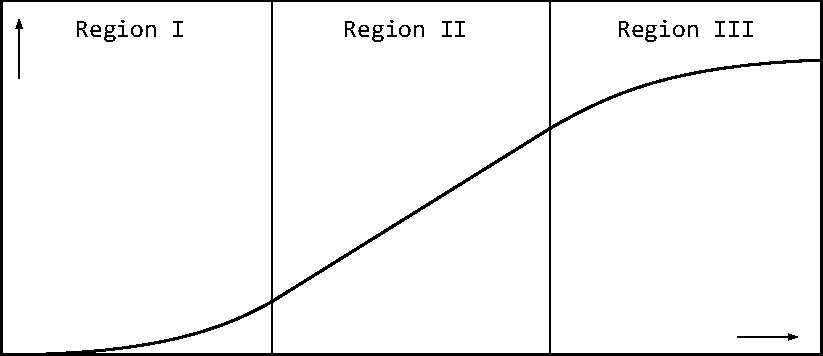
\includegraphics[width=.95\textwidth]{Pictures/CapillaryRise.pdf}
    \caption{Capillary rise dynamics as described in \cite{stange2003CapillaryDrivenFlow}}
    \label{fig: capillaryRise}
\end{figure}


As early as 1906, Bell and Cameron \cite{bell1906FlowLiquidsCapillary} empirically demonstrated a relationship $z^n=Kt$ with $n$ and $K$ as temperature-dependent constants. Lucas \cite{lucas1918UeberZeitgesetzKapillaren} in 1918 and Washburn \cite{washburn1921DynamicsCapillaryFlow} in 1921 independently derived an equation, neglecting the gravitational and inertial terms from Equation \ref{eq: NewtonDynCapillary}. They predicted a growth relationship for the meniscus as $z(t)\sim \sqrt{t}$.

Assuming Poiseuille flow, for a tube with a constant diameter, the fluid velocity can be written as:
\begin{equation}
    \frac{dl}{dt}= \frac{\sum \Delta p}{8r^{2}\eta z}(r^{4}+ 4\epsilon r^{3})
\end{equation}
with $\epsilon$ as the coefficient of slip and $\Delta p$ as the effective pressure acting to set the liquid in motion. This can be divided into three contributions:
\begin{itemize}
    \item atmospheric pressure $p_A$
    \item hydrostatic pressure $p_H$
    \item capillary pressure $p_C$
\end{itemize}
Assuming a horizontal capillary and constant atmospheric pressure, the Lucas-Washburn equation becomes:
\begin{equation}
    z(t)=\sqrt{\frac{r\cos\theta \sigma}{2\eta}t}
\end{equation}
The contact angle used here is typically the equilibrium contact angle. However, there have been attempts to improve the prediction of this equation by using the dynamic contact angle. \todo{citations!}
As already described in Chapter \ref{chap: BibliographyReview}, Bosanquet\cite{bosanquet1923LVFlowLiquids} and Quéré\cite{quere1997InertialCapillarity} have pointed out issues with this equation. Bosanquet has...
